
\section*{Общая характеристика работы}

\newcommand{\actuality}{\underline{\textbf{\actualityTXT}}}
\newcommand{\progress}{\underline{\textbf{\progressTXT}}}
\newcommand{\aim}{\underline{{\textbf\aimTXT}}}
\newcommand{\tasks}{\underline{\textbf{\tasksTXT}}}
\newcommand{\novelty}{\underline{\textbf{\noveltyTXT}}}
\newcommand{\influence}{\underline{\textbf{\influenceTXT}}}
\newcommand{\methods}{\underline{\textbf{\methodsTXT}}}
\newcommand{\defpositions}{\underline{\textbf{\defpositionsTXT}}}
\newcommand{\reliability}{\underline{\textbf{\reliabilityTXT}}}
\newcommand{\probation}{\underline{\textbf{\probationTXT}}}
\newcommand{\contribution}{\underline{\textbf{\contributionTXT}}}
\newcommand{\publications}{\underline{\textbf{\publicationsTXT}}}

{\actuality}
Исследования кинетических явлений (процессы переноса, оптические свойства) в квантовых системах с пониженной размерностью в настоящее время продолжают привлекать внимание, как теоретиков, так и экспериментаторов. Это связано с тем, что энергетический спектр электронов и дырок в таких системах из-за размерного квантования принципиальным образом отличается от объемного материала. Одним из наиболее перспективных в использовании и интенсивно изучаемых является эффект размерного квантования. Квантование движения частиц имеет место, когда характерный размер системы близок по величине к длине волны де Бройля носителей. Уменьшение размеров системы в одном, либо двух, трех направлениях приводит к тому, что движение частицы становится соотвественно квазидумерным, квазиодномерным или квазинульмерным. В настоящее время существует большое число видов низкоразмерных систем: квантовые ямы (КЯ), сверхрешетки (СР), квантовые проволоки (КП), квантовые доты (точки) и их системы. Именно появление размерно-квантованных зон проводимости (как и валентных зон) создает новые каналы поглощения и люминесценции, определяемые, например, переходом заряженной частицы между размерно-квантованными зонами проводимости (межподзонные переходы). При этом, что является очень важным, из-за локализации носителей сила осциллятора при таких переходах велика, что приводит к большим, порядка $10^3\,\text{cm}^{-1}$, значениям коэффициента поглощения слабой электромагнитной волны в далекой инфракрасной области спектра. Если в объемных полупроводниковых материалах электронные явления переноса определяются в основном рассеянием носителей на колебаниях кристаллической решетки, при низких температурах --- рассеянием на легированной примеси, то в размерно-ограниченных системах (квантовые ямы, гетероструктуры, квантовые проволоки и т.д.) возникает новый тип рассеяния – рассеяние носителей на шероховатой поверхности. Любое незначительное изменение размеров квантовой системы (например ширины КЯ, радиуса КП) приводит, естественно, к изменению энергии размерного квантования. Именно это изменение можно рассматривать как результат взаимодействия носителей с шероховатой поверхностью. Наиболее удачным для описания таких процессов рассеяния носителей является модель, когда размеры наноструктуры при движении заряженных частиц вдоль поверхности меняются случайным образом. В дальнейшем при описании кинетических явлений в размерно-ограниченных системах используется эта модель. Именно этот механизм рассеяния может описать большие значения подвижности носителей в области низких температур, наблюдаемые в экспериментальных исследованиях. При этом, естественно, чем меньше ширина размерно-квантованной системы, тем процессы рассеяния носителей на шероховатой поверхности становятся более активными. Поэтому механизм рассеяния носителей на шероховатой поверхности можно экспериментально выделить от других механизмов рассеяния по резкой зависимости кинетических коэффициентов от размеров наноструктуры и по влиянию поперечного электрического поля на процессы рассеяния. Эти процессы рассеяния влияют на кинетические явления по-разному в зависимости от ориентации напряженности внешнего однородного магнитного поля по отношению к оси пространственного квантования. Рассматриваемые процессы рассеяния важны в нелегированных наноструктурах в области низких температур $T$, потому что с ростом $T$ вначале важную роль начинают играть процессы рассеяния носителей на длинноволновых (акустических) колебаниях кристаллической решетки, а потом включаются процессы, связанные с взаимодействием заряженных частиц с оптическими фононами.

В настоящее время для описания кинетических явлений в размерно-ограниченных системах используется модель, в которой потенциал квантовой системы аппроксимируется параболой. Системы с квадратичным потенциалом интересны тем, что проявление эффектов размерного квантования в них происходит в достаточно больших размерно-ограниченных системах. Например, для типичных параметров параболической квантовой ямы GaAs/AlAs шаг пространственного квантования для электронов равен $14.6/a$ eV ($a$-ширина КЯ в $\AA$), т.е. при $a=10^3 \AA, \hbar\omega_e = 14.6 \text{ meV}$. Следовательно, уже при температуре $T=100 K$, должно заметно проявляться влияние размерно-квантованных уровней на кинетические свойства таких систем. Квадратичная зависимость потенциала также удобна для теоретических расчетов и позволяет получить многие характеристики полупроводниковых систем в аналитическом виде, что делает более удобным проводить детальный анализ рассматриваемых физических явлении.

В первой главе данной диссертационной работы представлен обзор экспериментов и теоретических работ, посвященных исследованию влияния процессов рассеяния носителей на шероховатой поверхности на оптические свойства и явления переноса в размерно-ограниченных системах. В ней же кратко изложена теория рассеяния носителей на шероховатой поверхности в размерно-ограниченных системах. Обсуждаются приближения, которые используются ниже в оригинальных главах диссертации.

Вторая глава диссертации посвящена расчету коэффициента поглощения света различной поляризации, позволяющий исследовать частотную зависимость поглощения света в широкой области частот и последовательно описать, как межподзонное, так и внутризонное поглощение с учетом взаимодействия электрона с шероховатой поверхностью.
В этой же главе исследуется влияние резонансного инфракрасного лазерного излучения на межзонное поглощение света в системах с пониженной размерностью (квантовые ямы, нанопроволоки), когда частота лазерного излучения равна или частоте размерного квантования или гибридной частоте.

В третьей главе диссертации проведено исследование влияния рассеяния носителей на шероховатой поверхности на процессы переноса в квантовых ямах и квантовых проволоках. Теоретические результаты сравниваются с экспериментальными данными в КЯ GaAs-AlAs, нанопроволоках Bi.

Четвертая глава диссертации посвящена исследованию явлений переноса (подвижность, термоэдс) в электрическом поле, направленном перпендикулярно оси размерно-ограниченной системы. В частности, показано, что подвижность с ростом напряженности поперечного электрического поля уменьшается, а в случае вырожденного электронного газа подвижность описывается осцилляционной кривой. Указанные особенности в подвижности возникают только при учете рассеяния носителей на шероховатой поверхности исследуемой наноструктуры.

%% {\progress} 
%% Этот раздел должен быть отдельным структурным элементом по
%% ГОСТ, но он, как правило, включается в описание актуальности
%% темы. Нужен он отдельным структурынм элемементом или нет ---
%% смотрите другие диссертации вашего совета, скорее всего не нужен.
%
%{\aim} данной работы является \ldots
%
%Для~достижения поставленной цели необходимо было решить следующие {\tasks}:
%\begin{enumerate}
%  \item Исследовать, разработать, вычислить и~т.\:д. и~т.\:п.
%  \item Исследовать, разработать, вычислить и~т.\:д. и~т.\:п.
%  \item Исследовать, разработать, вычислить и~т.\:д. и~т.\:п.
%  \item Исследовать, разработать, вычислить и~т.\:д. и~т.\:п.
%\end{enumerate}
%
%
%{\novelty}
%\begin{enumerate}
%  \item Впервые \ldots
%  \item Впервые \ldots
%  \item Было выполнено оригинальное исследование \ldots
%\end{enumerate}
%
%{\influence} \ldots
%
%{\methods} \ldots
%
%{\defpositions}
%\begin{enumerate}
%  \item Первое положение
%  \item Второе положение
%  \item Третье положение
%  \item Четвертое положение
%\end{enumerate}
%
%{\reliability} полученных результатов обеспечивается \ldots \ Результаты находятся в соответствии с результатами, полученными другими авторами.


{\probation}
Основные результаты работы докладывались~на:
перечисление основных конференций, симпозиумов и~т.\:п.

%{\contribution} Автор принимал активное участие в обсуждении и постановке задач, рассмотренных в диссертационной работе. Все основные оригинальные расчеты проведены автором самостоятельно.

%\publications\ Основные результаты по теме диссертации изложены в ХХ печатных изданиях~\cite{Sineavsky2006,Karapetyan2006,Karapetyan2011,Karapetyan2012,Solovenko2012,Karapetyan2014,Karapetyan2017},
%Х из которых изданы в журналах, рекомендованных ВАК~\cite{Sineavsky2006,Karapetyan2006,Karapetyan2011,Karapetyan2012,Solovenko2012,Karapetyan2014,Karapetyan2017}, 
%ХХ --- в тезисах докладов~\cite{Lermontov,Management}.

\ifthenelse{\equal{\thebibliosel}{0}}{% Встроенная реализация с загрузкой файла через движок bibtex8
    \publications\ Основные результаты по теме диссертации изложены в XX печатных изданиях, 
    X из которых изданы в журналах, рекомендованных ВАК, 
    X "--- в тезисах докладов.%
}{% Реализация пакетом biblatex через движок biber
%Сделана отдельная секция, чтобы не отображались в списке цитированных материалов
    \begin{refsection}%       
        \printbibliography[heading=countauthorvak, env=countauthorvak, keyword=biblioauthorvak, section=1]%
        \printbibliography[heading=countauthornotvak, env=countauthornotvak, keyword=biblioauthornotvak, section=1]%
        \printbibliography[heading=countauthorconf, env=countauthorconf, keyword=biblioauthorconf, section=1]%
        \printbibliography[heading=countauthor, env=countauthor, keyword=biblioauthor, section=1]%
        \publications\ Основные результаты по теме диссертации изложены
       в \arabic{citeauthor} печатных изданиях,
       \arabic{citeauthorvak}~из которых изданы в журналах,
       рекомендованных ВАК, \arabic{citeauthorconf}~в тезисах
       конференций.\nocite{Karapetyan2006,Sineavsky2006,Karapetyan2011a,Karapetyan2012a,Solovenko2012,Karapetyan2014,Karapetyan2017,Minsk2008a,PGU2006,PGU2006,PGU2008,PGU2010,PGU2012,Ul2004,Ul2005,Tir2005,Orlando2005,CFM-2005,Ul2006,Ul2006,Saransk2006,Tir2007,Chisinau2007,Ul2008,Minsk2008,Ul2009,Tir2009,Chisinau2009,Kaluga2009,CFM-2009,Nanopiter-2010,Ul2010,Ul2011,Tir2011,Ul2012,Ul2013,Tir2013,Ul2015,Tir2015}.
    \end{refsection}
}
%При использовании пакета \verb!biblatex! для автоматического подсчёта
%количества публикаций автора по теме диссертации, необходимо
%их здесь перечислить с использованием команды \verb!\nocite!.
    

 % Характеристика работы по структуре во введении и в автореферате не отличается (ГОСТ Р 7.0.11, пункты 5.3.1 и 9.2.1), потому её загружаем из одного и того же внешнего файла, предварительно задав форму выделения некоторым параметрам

%Диссертационная работа была выполнена при поддержке грантов ...

%\underline{\textbf{Объем и структура работы.}} Диссертация состоит из~введения, четырех глав, заключения и~приложения. Полный объем диссертации \textbf{ХХХ}~страниц текста с~\textbf{ХХ}~рисунками и~5~таблицами. Список литературы содержит \textbf{ХХX}~наименование.

%\newpage
\section*{Общая характеристика работы}
{\actuality} Актуальность исследований
Исследования кинетических явлений (процессы переноса, оптические свойства) в наносистемах продолжают привлекать внимание как теоретиков, так и экспериментаторов. Это связано с тем, что энергетический спектр носителей в таких системах (движение электронов вдоль ширин квантовой ямы, вдоль радиуса квантовой проволоки являются финитными) принципиальным образом отличаются от объемных материалов.
Именно появление размерно-квантованных зон проводимости (как и валентных зон) создает новые каналы поглощения и люминесценции света, что безусловно расширяет возможности приборного приложения таких квантовых систем в оптоэлектронике. Изучение процессов рассеяния носителей на шероховатой поверхности является важным и актуальным, так как позволяет понять большие значения подвижности, экспериментально наблюдаемые в тонких наноструктурах, объяснить большие (порядка $10^3$см$^{-1}$) значения коэффициента поглощения слабой электромагнитной волны в инфракрасной области спектра. При низких температурах и тонких нелегированных наносистемах рассеяние носителей на шероховатой поверхности может оказаться доминирующим механизмом рассеяния, определяющим физические свойства квантовых систем. Заметное влияние внешних полей (например поперечного электрического поля) на процессы рассеяния носителей на шероховатой поверхности представляются перспективным для создания различных приборов из наноструктур, кинетическими процессами в которых можно управлять.
Таким образом, исследования кинетических явлений в размерно-ограниченных системах являются перспективными и актуальными.

\underline{\textbf{Связь работы с научными программами, планами, темами}}
Диссертационная работа выполнялась по планам кафедры теоретической физики и научно исследовательской лаборатории “Полярон” Приднестровского государственного университета им Т.Г. Шевченко, а так же по научному плану лаборатории физической кинетики ИПФ АН Молдовы. Некоторые разделы работы выполнены в рамках Украинского научно-технического центра (грант №5062), STCU (грант №5929)

\underline{\textbf{Цель и задачи исследования}}
Основной задачей диссертационной работы является теоретическое исследование влияния процессов рассеяния носителей на шероховатой поверхности наноструктуры во внешних полях (поперечных электрическом и магнитном полях) не оптические свойства и процессы переноса заряда (подвижность, темроэдс) в размерно-ограниченных системах (квантовые ямы, нанопроволоки)

\underline{\textbf{Решены следующие задачи}}
\begin{itemize}
\item Теоретически исследованы процессы рассеяния носителей на рероховатой поверхности в размерно-ограниченных системах (квантовые ямы (КЯ), нанопроволоки (КП) в модели параболического потенциала во внешних электрическом и магнитном полях.
\item Подробно изучено влияние поперечных электрического и магнитного полей на процессы переноса заряда (подвижность, термоэдс) в наноструктурах с учетом рассеяния носителей на шероховатой поверхности.
\item Исследовано влияние ИК лазерно излучения на межзонное погшлощение слабой электромагнитной волны в нанопровлоках, когда частота излучения равна частоте размреного квантования (размерно-индуцированный разеонанс) или гибридной частоте (магнитно-инфракрасный резонанс)
\item Выяснена роль процессов рассеяния на шероховатой поверхности на внутризонные, межзонные и межподзонные оптические переходы в размерно-ограниченных системах.
\end{itemize}

\underline{\textbf{Научная новизна}}
\begin{enumerate}
	\item Из общих соотношений неравновесной квантовой статистики в приближении времени релаксации вычисляется электропроводность в размерно-ограниченных системах (прямоугольные, параболические квантовые ямы, нанопроволоки) с одновременным учетом рассеяния носителей на шероховатой поверхности и упругого рассеяния на длинноволновых (акустических) колебаниях. Полученные теоретические результаты по величине подвижности, по зависимости подвижности от температуры,  от размеров наноструктуры находят экспериментальное подтверждение в разнообразных квантовых системах. Именно сравнение теоретических результатов с экспериментальными данными позволяет провести оценки параметров флуктуирующей поверхности наноструктуры. Сформулированны условия на размеры квантовых наносистем, температуру, когда упругие процессы рассеяния электронов на шероховатой поверхности становятся доминирующими по сравнению с рассеянием носителей на акустических фононах.
	\item Подробно исследовано влияние однородного магнитного поля $\vect{H}$ на электропроводность в размерно квантованных системах (квантовые ямы, параболические нанопроволоки) с учетом рассеяния носителей на шероховатой поверхности. Показано, что с ростом напряженности продольного магнитного поля подвижность увеличивается, что связано с уменьшением радиуса локализации носителей тока в исследуемых наноструктурах, т.е. к уменьшению вероятности рассеяния носителей на шероховатой поверхности. В поперечном магнитном поле подвижность с ростом напряженности поля уменьшается. Такое поведение подвижности от $\vect{H}$ связано с тем, что в скрещенных электрическом и магнитном полях носители с дрейфовой скоростью перемещаются вдоль оси пространственного квантования, поэтому активно участвуют в процессах рассеяния на шероховатой поверхности исследуемой наноструктуры. Некоторые теоретические результаты сравниваются с экспериментальными данными для электропроводности в магнитном поле для нанопроволок Bi
	\item Впервые исследовано влияние интенсивного лазерного излучения на межзонное поглощение слабой электромагнитной волны в квантовых проволоках. Показано, что когда частота лазерного излучения равна или частоте размерного квантования (размерно-инфракрасный резонанс) или, в присутствии поперечного магнитного поля, гибридной частоте (магнито-инфракрасный резонанс) то лазерная подсветка определяет форму осцилляций коэффициента поглощения света. В частности показано, что второй пик магнетопоглощения расщепляется на два пика, полуширина которых и расстояние между которыми зависят от интенсивности резонансного лазерного излучения. Проведено подробное исследование динамики изменения частотной зависимости коэффициента межзонного поглощения света при увеличении интенсивности резонансного лазерного излучения. Именно существенное изменение частотной зависимости коэффициента межзонного поглощения света в поле резонансного лазерного излучения дает возможность наблюдать заметное поглощение света при частотах, когда в отсутствии лазерной подсветки исследуемая квантовая система не поглощает электромагнитную волну.
	Важно отметить, что заметное влияние лазерного излучения на оптические характеристики размерно-ограниченных систем осуществляется при небольших (экспериментально достигаемых) интенсивностях ИК излучения, что позволяет надеяться на экспериментальное обнаружение предсказанного эффекта. Именно в квантованных нанопроволоках, из-за одномерного движения носителей, возникают особенности в плотности электронных состояний, что приводит к наиболее яркому проявлению влияния резонансного лазерного излучения на оптические характеристики исследуемой квантовой системы.
	\item Впервые проведены теоретические исследования электропроводности, термоэдс в размерно-квантованных системах (параболические квантовые ямы, параболические нанопроволоки) в присутствии однородного электрического поля $\vect{E}$, направленного вдоль оси пространственного квантования. 
	Показано, что только при учете взаимодействия носителей с шероховатой поверхностью, подвижность, термоэдс с ростом $\vect{E}$ уменьшаются. В случае вырожденного электронного (дырочного) газа подвижность, термоэдс осциллируют при изменнии поперечного однородного электрического поля. Предложена физическая интерпретация такого поведения кинетических коэффициентов от  $\vect{E}$. Проведены детальные исследования влияния однородного магнитного поля различной ориентации по отношению к $\vect{E}$ на подвижность квантовых проволок Bi.
\end{enumerate}

{\defpositions}
\begin{enumerate}
\item Результаты теоретических исследований влияния внешних электрического и магнитного полей на процессы рассеяния носителей на шероховатой поверхности в наноструктурах (квантовые ямы, квантовые проволоки) с параболическим потенциалом. Сформулированы условия на температуру и размеры квантовй системы когда процессы рассеяния на шероховатой поверхности являются доминирующими в нелегированных размерно-ограниченных системахю
\item Влияние электрического поля, направленного перпендикулярно поверхности размерно-ограниченной квантовой системы и магнитного поля на процессы переноса заряда (подвижность, теромэдвс) при учете процессов рассеяния носителей на шероховатой поверхности.
\item Исследования помежзонному поглощению слабой электромагнитной волны в параболических квантовых проволоках в поле ИК лазлерного излучения, частота которого равна или частоте размерного квантования (размерно-инфракрасный резонанс) или гибридной частоте (магнитно-инфракрасный резонанс).
\item Исследования особенностей коэффициента поглощения света различной поляризации при межподнонных, внутризонных переходах с учетом взаимодействия носителей с шероховатой поверхностью в квантовых ямах в широкой области частот.
\end{enumerate}

\section*{Основное содержание диссертации}

Глава 1. Рассеяние носителей на шероховатой поверхности

В 1.1. дан обзор основных теоретических и экспериментальных работ, исследовавших влияние процессов рассеяния носителей на шероховатой поверхности н акинетические явления в размерно-ограниченных системах (квантовые ямы, нанопроволоки). Именно эти работы убедительно указывают на важность и актуальность исследований таких процессов рассеяния заряженных частиц в квантовых системах.

В 1.2 первой главы рассмотрена теория рассеяния носителей на шероховатой поверхности в размерно-ограниченных системах. Приведены результаты расчетов времени релаксации носителей с учетом их рассеяния на шероховатой поверхности, определяемое квантово-механической вероятностью рассеяния в единицу времени, для случая двумерного электронного газа (квантовые ямы), одномерного электронного газа (квантовые проволоки), для гауссовой и $\delta$-образной флуктуации поверхности. Особое внимание уделяется расчету времени релаксации $\tau_\alpha$ во внешнем постоянном электрическом поле $\vect{E}$, направленном вдоль оси пространственного квантования низкоразмерной системы с праболическим потнециалом.
В случае $\delta$-образной флуктуации поверхности для параболической квантовой ямы обратное время релаксации, связанное с рассеянием электрона с эффективной массой $m_e$ на шероховатой поверхности, описывается соотношением: 
\begin{equation} \label{eq:syn_01}
\frac{1}{\tau _{\alpha } } =\frac{\gamma_0 m_e (\hbar\omega)^2 }{\hbar^3 a^2 } \left[\left(n+\frac{1}{2} \right)+N_c \right]^2, \;
N_c =\frac{e^2 E^2 }{\hbar m_e \omega^3 } .
\end{equation}  
$\gamma_0 m_e$ --- высота флуктуации, $\hbar\omega$ --- энергия размерного квантования, которая простым образом связана с величиной потенциальной энергии $\Delta E_c$ на границе параболической квантовой ямы с шириной $a$.
\[
\hbar\omega = \frac{2\hbar}{a}\left(  \frac{2\Delta E_c}{m_e} \right)^{\frac{1}{2}} 
\]
Важно отметить, что зависимость времени релаксации от электрического поля представляется важным, так как при других механизмах рассеяния (на длинноволновых акустических фононах, на примесях) $\tau_\alpha$ не зависит от величины поперечного электрического поля. Заметим, что $\tau_\alpha$ (для любого типа флуктуации) совпадает с транспортным временем релаксации, используемому при решении уравнения Больцмана.
Заметим, что $\tau_\alpha$ определяется только номером размерно-квантованной зоны проводимости, в которой происходит рассеяние и с ростом $\vect{E}$ уменьшается, что является принципиально важным при исследовании кинетических явлений в размерно ограниченных системах. В этом же параграфе исследуется $\tau_\alpha$ в анизотропных параболических квантовых проволоках (такая модель часто применяется при описании кинетических явлений в нанопроволоках [???]  и находит свое математическое подтверждение [???], когда магнитное поле $\vect{H}$ параллельно постоянному электрическому полю $\vect{E}$, направленного перпендикулярно оси нанопроволоки. При этом обратное время релаксации, связанное с рассеянием электрона на шероховатой поверхности в нижайшей размерно-квантованной зоне проводимости имеет вид:
\begin{equation} \label{eq:syn_02}
\frac{1}{\tau_\alpha}=\frac{2m_e\Omega^2_e \gamma_0}{\hbar R^2 \left|k_x\right|} \left[\left(\frac{\omega}{\Omega_e}\right) \left(n+\frac{1}{2}\right)+ \left(m+\frac{1}{2}\right)+ \frac{2\Delta_c}{\hbar\Omega_e} \left(\frac{\omega}{\Omega_e}\right)^3\right]^2.
\end{equation}
$\Omega^2_e= \omega^2 + \omega_c^2$, $eH/m_e c$ --- соответственно гибридная и циклотронная частоты, $k_x$ --- волновой вектор электрона вдоль оси квантовой проволоки.

Глава 2. Влияние рассеяния носителей на шероховатой поверхности на оптические свойства размерно-ограниченных систем

В 2.1 рассмотрено межподзонное и внутризонное поглощение света в квантовых системах с пониженной размерностью с учетом рассеяния на шероховатой поверхности. В частности произведен расчет коэффициента поглощения слабой электромагнитной волны $K\left(\Omega \right)$ различной поляризации, как для внутризонных переходов , так и для межподзонных переходов с учетом взаимодействия электронов с шероховатой поверхностью в квантовой яме. При этом коэффициент поглощения электромагнитной волны вычисляется без использования теории возмущений по взаимодействию носителей с шероховатой поверхностью, что позволяет исследовать частотную зависимость $K(\Omega)$ в широкой области частот и сформулировать условия применимости теории возмущений и последовательно описать внутризонное поглощение света и при неслабых взаимодействиях электрона с шероховатой поверхностью.	

Расчет коэффициента поглощения света частоты $\Omega$ и вектора поляризации $\vect{\xi}$ проводился по формуле Кубо.
Матричные элементы оператора импульса  для прямоугольной квантовой ямы определяются соотношениями $(\alpha (n, \vect{k}{_\bot}), \; \beta (n', \vect{k}'_{\bot}))$:
\begin{equation} \label{eq:syn_04}
\left\langle \alpha \left| \hat{p}^{(z)} \right| \beta \right\rangle = \frac{2}{a} i\hbar \delta_{k_\bot k'_\bot} \frac{n n_1}{n^2 - n_1^2} \left[(-1)^{n+n_1} -1 \right] , \; n \neq n_1
\end{equation}
\begin{equation} \label{eq:syn_05}
\left\langle \alpha \left| \hat{p}^{(x)} \right| \beta \right\rangle = \hbar k_x \delta_{\alpha\beta},\;
\left\langle \alpha \left| \hat{p}^{(y)} \right| \beta \right\rangle = \hbar k_y \delta_{\alpha\beta}.
\end{equation} 
Из которых следует правило отбора для переходов электрона между размерно-квантованными зонами проводимости $n \neq n_1$, такое что поглощение света в данном случае, возможно только в ТМ–поляризации.

Для невырожденного электронного газа, коэффициент поглощения света, связанный с переходом электрона из нижайшей зоны проводимости $(n=1)$ в ближайшую размерно-квантованную зону проводимости $(n_1=2)$, записывается следующим образом $(\beta _0\hbar \Omega \gg 1)$:
\begin{equation} \label{eq:syn_6}
K(\Omega) = K_M \frac{1}{1+\left(\dfrac{\tau_0 }{17 \hbar} \Delta_0 \right)^2 } ;
\end{equation} 
\[
K_M =\frac{2^{12} e^2 a^5 n_e }{\hbar cn_0 \pi^5 \gamma_0 3^3 \cdot 17}, \;
\Delta_0 =\hbar \Omega -3\varepsilon_0.
\]
$n_e =N/L_x L_y $~---~поверхностная плотность электронов. При записи (\ref{eq:syn_6}) учитывалось, что в размерно-квантованной зоне, на которую происходит оптический переход носителя, электронов нет, поэтому $n_{\beta } \ll 1$. Последнее приближение вполне справедливо, если  $3\varepsilon_0 \gg kT$, т.е. почти все электроны находятся на нижайшей размерно-квантованной зоне проводимости $(n=1)$, и, следовательно, $\sum n_{k_{\bot } } \cong N$ ($N$~---~число электронов в исследуемой квантовой системе). Из \eqref{eq:syn_6} следует, что частотная зависимость коэффициента поглощения света описывается резонансной кривой с полушириной  $\delta =17\cdot 2\hbar /\tau_0 $. Величина коэффициента поглощения электромагнитной волны при рассматриваемом механизме рассеяния существенным образом определяется толщиной квантовой ямы $\left(K_M \sim a^5 \right)$ и не зависит от температуры. $K\left(\Omega \right)$  в максимуме при $n_e =4\cdot 10^{11} \text{cm}^{-2} $, $n_0 = 3.2$,   принимает значение   $K_M^{\left(\delta \right)} =0.25\cdot a_0^5 /\gamma_0 $ ($a_0 $, $\sqrt[4]{\gamma_0}$~--–~измеряются в ангстремах), т.е. при  $a_0 = 80 \AA$,  $\sqrt[4]{\gamma_0} = 10 \AA$ (именно такие значения   хорошо описывают значения подвижности   экспериментально наблюдаемые в КЯ GaAs/AlGaAs, $K_M =2\cdot 10^4 \text{cm}^{-1} $. Большие значения коэффициента поглощения света позволяют надеяться на практическое использование таких размерно-квантованных систем в качестве детекторов ИК-излучения в области низких температур. Полуширина линии поглощения для рассматриваемого прямого оптического перехода при рассматриваемых выше параметрах $\delta =6.5\cdot 10^6 \left(\gamma_0 /a_0^6 \right)\text{meV}$. Следовательно, при  $a_0 = 60 \AA$,  $\sqrt[4]{\gamma_0} = 15 \AA$,  $\delta = 7 \text{ meV}$, что безусловно, находится в области экспериментального измерения.

Для ТЕ-поляризованного излучения, из \eqref{eq:syn_05} следует, что  возможно поглощение света только в одной размерно-квантованной зоне проводимости. Если рассматривать поглощение слабой электромагнитной волны в нижайшей $(n=1)$ размерно-квантованной зоне, то выражение для коэффициента поглощения света в случае невырожденного электронного газа принимает вид:
\begin{multline} \label{syn_7}
K(\Omega) = \frac{2 \pi e^2 n_e }{m_e c n_0 a \hbar \beta_0 \Omega^2} \int\limits_0^{\infty}x dx \int\limits_{-\infty}^{\infty}y dy \times \\
\times \exp{\left\lbrace  - 2\Gamma_0 |y| \left[ 1 - \frac{\delta_0}{\pi x |y|}\sin^2{\left( \frac{x|y|}{\delta_0}\right) } + \frac{1}{\pi} \mathrm{Si}{\left( \frac{2x|y|}{\delta_0}\right) } \right]  \right\rbrace   }.
\end{multline} 

Здесь введены следующие обозначения:
\[
\delta_0 = 2\hbar \Omega \beta_0,
\]
\[
\Gamma_0 = \pi^2 \left(\frac{\varepsilon_0}{\hbar \Omega} \right) \left( \frac{\gamma_0}{a^4} \right),
\]
\[
\mathrm{Si}(z) = -\frac{\pi}{2} + \int\limits_0^z{d\tau\frac{\sin{\tau}}{\tau}}.
\]

В случае низких температур выражение для поглощения света \eqref{21_09_14} можно записать:
\begin{equation} \label{eq:syn_8}
K(\Omega )=\frac{4\pi e^{2} n_{e} }{m_e c n_0 a \hbar\beta \Omega^2 } \frac{\Gamma_0 }{1+\Gamma_0^2 }
\end{equation} 

В нижайшем приближении по взаимодействию электрона с шероховатой поверхностью $\Gamma_0 \ll 1$, что соответствует обычной теории возмущений, из (\ref{eq:syn_8}) следует:
\begin{equation} \label{eq:syn_9}
K(\Omega )=\frac{2^4 e^2 n_e \gamma_0 m}{\pi c n_0 a\hbar^3 \beta_0 } \left(\frac{\varepsilon_0 }{\hbar\Omega } \right)^3
\end{equation} 

В рассматриваемом случае $K(\Omega )\sim \Omega^{-3} $ и при низких температурах ($T=50 K$) для $\gamma_0^{1/4} =15 \AA$, $n_e = 2\cdot 10^{12} \text{cm}^{-2} $, $a=50 \AA$, $K_0 (\Omega )\cong 10\left(\varepsilon_0 / \hbar\Omega \right)^3 \text{cm}^{-1} $.

При $\Gamma_0 \gg 1$, что соответствует сильному взаимодействию электрона с шероховатой поверхностью, коэффициент внутризонного поглощения электромагнитной волны определяется соотношением:
\begin{equation} \label{eq:syn_10}
K(\Omega )=\frac{2^4 e^2 n_e a}{\pi^3 cn_0 \hbar } \frac{1}{\delta_0 } \left(\frac{a^4 }{\gamma_0 } \right)
\end{equation} 

В рассматриваемом приближении сильной связи $a^4 /\gamma_0 =1$, $K(\Omega )\sim \Omega ^{-1} $ и для $\delta_0 =10$, $a=50 \AA$, $K(\Omega )\cong 120 \text{ cm}^{-1} $. Следовательно, в области низких частот для узких квантовых ям с большой флуктуацией поверхности теория возмущений при исследовании внутризонного поглощения света может оказаться несправедливой.

В 2.2 и 2.3 исследовалось влияние резонансного лазерного излучения на оптические свойства квантовых ям и квантовых проволок.

Для квантовых ям получен коэффициент межзонного поглощения слабого света, в случае когда частота лазерного излучения $\omega $ равна частоте размерного квантования $\omega_c $ в зоне проводимости (размерно-инфракрасный резонанс -- РИР), а напряженность $E$ постоянного электрического поля направлена параллельно поверхности параболической квантовой ямы (ПКЯ): 
\begin{multline} \label{eq:syn_11} 
K(\Omega )=K_0 \sum _{n} \, V_n^2 \times  \\
\times \left\{\frac{\pi }{2} +\int_0^{\infty } dt \exp \left(-\frac{x^2 }{2} \right)L_n \left(x^2 \right)\frac{\sin \left[x\left(\Delta_n -\delta x^2 \right)\right]}{x} \right\}
\end{multline} 
где 
\[\Delta_n =\frac{\hbar \Omega -E_g -\hbar \omega^* \left(n+{\tfrac{1}{2}} \right)}{\hbar \sqrt{\gamma } } ; \; \omega^* =\omega_c +\omega_v ;\] 
$\hbar \omega_v $~---~энергия размерного квантования в валентной зоне, $V_n $~---~матричный элемент волновых функций электрона в зоне проводимости и в валентной зоне для ПКЯ. В частном случае 
\[V_0 =\mathop{\left(\lambda_c \lambda_v \right)}\nolimits^{{\tfrac{1}{4}} } \sqrt{\frac{2}{\lambda_c +\lambda_v } } ;\; \; V_1 =2\sqrt{2} \frac{\mathop{\left(\lambda_c \lambda_v \right)}\nolimits^{{\tfrac{3}{4}} } }{\mathop{\left(\lambda_c +\lambda_v \right)}\nolimits^{{\tfrac{3}{2}} } } ;\; \; \lambda_i =\frac{m_i \omega^i }{\hbar } (i=c,v).\] 
Для типичных параметров ПКЯ GaAs-AlGaAS $\lambda_c /\lambda_v =0.47$ ($m_c =0.06m_0 ,$ $m_v =0.4m_0 $). Постоянное продольное электрическое поле существенным образом влияет на межзонный коэффициент поглощения света. При этом в электрическом поле возможно заметное поглощение в длинноволновой области спектра, а в высокочастотной области поглощение света определяется характерной осцилляционной зависимостью от частоты. С ростом напряженности постоянного электрического поля осцилляции становятся наиболее отчетливыми.

Для квантовых проволок получен коэффициент поглощения света, связанный с переходом электрона из нижайшей валентной зоны $(m=n=0)$ в нижайшую размерно-квантованную зону проводимости $(n=m=0)$, который имеет следующий вид:
\begin{equation} \label{eq:syn_12}
K\left(\Omega\right)=K_0\sum_{nm}{ {\lvert\langle \alpha_c | \alpha_v \rangle\rvert}^2 {\left[\frac{8\pi \mu^*\omega_f}{\hbar a}\right]}^{\frac{1}{2}} \mathrm{Re} \int\limits_0^\infty {dx e^{f^2\left(x\right)}\left[1-\Phi \left(f\left(x\right)\right)\right]}}
\end{equation}
\[
\Phi \left(z\right)=\frac{2}{\sqrt{\pi}}\int\limits_0^z {e^{-\tau^2}}d\tau ,
\] 
\[
f\left(x\right)={\left(\frac{\omega^2_f}{4a}\right)}^{\frac{1}{2}}\frac{1}{x}\left[1-ix\left(\frac{\Delta }{\hbar \omega_f}-x^2\right)\right],\; \Delta =\hbar \Omega-E^*_g .
\] 

При $\omega^2_f / 4a \ll 1$, то форма линии межзонного поглощения света (высота, полуширина) полностью определяется интенсивностью лазерного излучения, и коэффициент поглощения света согласно \eqref{eq:syn_12} записывается следующим образом :
\begin{equation} \label{eq:syn_13}
K(\Omega)=K_0 {\lvert\langle \alpha_c | \alpha_v \rangle\rvert}^2
{\left[\frac{\pi {\mu }^*\left|\Delta \right|}{{\hbar }^2a}\right]}^{\frac{1}{2}}
\begin{cases}
e^{-z} \mathrm{K}_{1/4}(z), \Delta \le 0 \\ 
\frac{\pi }{\sqrt{2}}e^{-z}[\mathrm{I}_{{1}/{4}}\left(z\right)+\mathrm{I}_{-1/4}\left(z\right)], \Delta >0
\end{cases}
\end{equation}
\[
z=\frac{\Delta^2}{8a\hbar^2}=\frac{1}{2}\left(\frac{\Delta}{\hbar\omega_f} \right)^2 \left(\frac{\omega_f^2}{4a} \right),
\]
$\mathrm{K}_v\left(z\right)$~---~функция Макдональда, $\mathrm{I}_v\left(z\right)$~---~модифицированная функция Бесселя.
С ростом интенсивности ИК излучения ($\xi $ уменьшается при фиксированном значении $\omega_f$) форма линии поглощения изменяется: величина максимума поглощения уменьшается, а полуширина увеличивается. Заметим, что уже при $\xi \le 1$ коэффициент межзонного поглощения света полностью определяется интенсивностью ИК лазерного излучения.

В случае межзонное поглощение света в области второго пика $m=0$, $n=1$ $\left( L_1\left(2at^2\right)=1-2at^2 \right)$ коэффициент поглощения света при $\xi ={{\omega }^2_f}/{4a}<1$ (форма линии поглощения определяется интенсивностью резонансного ИК излучения) принимает следующий вид:
\begin{multline} \label{eq:syn_14}
K\left(\Omega\right)=K_0{\left|\left\langle \widetilde{\alpha }_c |\widetilde{\alpha }_v\right\rangle \right|}^2 \pi z{\left[\frac{2^* \pi }{\hbar }{\left(\frac{8z}{a}\right)}^{1/2}\right]}^{1/2}e^{-z}\times\\
\times \left\{-\left[I_{3/4}\left(z\right)+\mathrm{sign}(\Delta) I_{-3/4}\left(z\right)\right]+\left(1+\frac{1}{4z}\right)\left[(I_{-1/4}\left(z\right)+ \mathrm{sign}(\Delta)  I_{1/4}\left(z\right)\right]\right\}
\end{multline}
\[
\mathrm{sign}(\Delta) = \begin{cases}
1,&\Delta >0 \\ 
-1,&\Delta <0
\end{cases}
\] 
$\left\langle \widetilde{\alpha }_c |\widetilde{\alpha }_v \right\rangle$ --- матричный элемент сглаженных волновых функций носителей в возбужденном состоянии валентной зоны ($m=0$, $n=1$) и в первом возбужденном состоянии размерно-квантованной зоны проводимости.
С ростом напряженности $E$ электрического поля пик магнетопоглощения деформируется и при $\xi \ll 1$ расщепляется на два пика. При этом расстояние между ними и их полуширина увеличивается. Расщепление второго пика поглощения связано с тем, что при $\omega_L=\Omega_e$ возбужденное гибридное состояние $(n=1)$ двукратно вырождено, и при взаимодействии с ИК лазерным излучением оно расщепляется. Эта ситуация близка к двойному оптическому резонансу (ДОР) на межзонных переходах в объемных материалах.
Заметим, что $n$-пик магнетопоглощения расщепляется на $n$ пиков.

Пусть при некотором значении напряженности электрического поля $E_c$ интенсивной электромагнитной волны вклад лазерного излучения в полуширину магнетоосцилляций примерно такой же как вклад, определяемый рассеянием носителей на шероховатой поверхности $(\xi =1)$. Естественно при $E_c<E$ форма линии межзонного поглощения слабой электромагнитной волны полностью определяется внешней лазерной подсветкой. Для типичных параметров полупроводниковой нанопроволоки $m_e=0.06m_0$, $m_v=0.4m_0$, $\sqrt[3]{\gamma_0}=20\ \AA $ (такое значение $\sqrt[3]{\gamma_0}$ хорошо описывает большие значения подвижности $\mu \propto 10^4\ \frac{cm^2}{V\cdot s}$, характерные для квантовых проволок) при $R_0=10^3\ \AA $, $E_c= 7\ \frac{V}{cm}$ для лазера $\mathrm{H_2 O}$ $\left(\hbar {\omega }_L=0.044\ eV\right)$. Следовательно, резонансное лазерное излучение заметно влияет на частотную зависимость межзонного поглощения света при небольших, вполне экспериментально доступных значений интенсивности ИК- лазерного излучения.

Глава 3. Влияние шероховатой поверхности на кинетические эффекты в низкоразмерных системах
В данной главе делается попытка объяснить особенности температурной зависимости электропроводности, экспериментально наблюдаемые в нелегированных наноструктурах, учитывая процессы рассеяния носителей на шероховатой поверхности и на фононах. Именно из сравнения теоретических результатов с экспериментальными данными по температурной зависимости электропроводности можно провести оценки параметров флуктуирующей поверхности. Учет двух механизмов рассеяния позволил сформулировать условия на ширину размерно-ограниченной системы и температуру, когда рассеяние носителей на шероховатой поверхности преобладает над рассеянием на фононах.

Для прямоугольной КЯ с бесконечным потенциалом с гауссовой флуктуацией поверхности при низких температурах  $3\hbar^2 \pi^2 /\left(2m_e L^2 \right) \gg k_0 T$, когда электроны находятся на нижайшем размерно-квантованном уровне $(n=1)$ прямоугольной КЯ получено выражение для электропроводности:
\begin{equation} \label{eq:syn_15}
\sigma _{xx} =\frac{e^2 \hbar^3 \delta}{m_e^2 \pi^2 \left(\Delta \Lambda^2 V_1 \right)^2 L} \int\limits_0^\infty { \frac{d\tau \cdot \tau \cdot \exp \left(\delta \tau -\beta_0 \tilde{\xi }\right)}{\exp(-\tau )\mathrm{I}_0 (\tau )\cdot \left[\exp \left(\delta \tau -\beta_0 \tilde{\xi }\right)+1\right]^2 }},
\end{equation}
\[
\beta_0 = \frac{1}{k_0 T}, \; \delta =\frac{\beta_0 \hbar^2 }{m_e \Lambda^2 },
\] 
$\tilde{\xi }=\xi -\varepsilon _{1} $ --- химический потенциал, отсчитанный от дна нижайшей размерно-квантованной зоны проводимости,
\begin{equation} \label{eq:syn_16}
\beta_0 \tilde{\xi }=\ln\left[\exp\left(\frac{\beta_0 \pi \hbar^2 n_s }{m_e} \right)-1\right].
\end{equation}
$n_s $~---~поверхностная плотность электронного газа.

Из выражения \eqref{eq:syn_15} следует, что подвижность существенным образом зависит от толщины размерно-квантованной системы $(\mu_0 \sim L^6 )$. При низких $T$ $(\delta \gg 1)$ подвижность практически не зависит от температуры и при высоких температурах $(\delta <1)$ с ростом $T$ увеличивается. Такое поведение подвижности от $L$ и $T$ экспериментально наблюдалось в GaAs/AlAs \cite{Sakaki1987}. При низких температурах подвижность определяется только размером КЯ и параметрами флуктуирующей поверхности $\Delta $, $\Lambda $. При изменении толщины КЯ от $70 \AA$ до $100 \AA$ подвижность изменяется от $\mu_0 =2.6\cdot 10^3 \text{cm}^2 / \text{Vs}$ до $\mu_0 =2\cdot 10^4 \text{cm}^2 /\text{Vs}$, что согласуется с экспериментальными данными в КЯ GaAs/AlAs \cite{Sakaki1987}.

При учете двух механизмов рассеяния (рассеяние на шероховатой поверхности и на акустических фононах), получено выражение для электропроводности:

\begin{equation} \label{eq:syn_17}
\sigma _{xx} =\frac{\beta_0 e^2 }{Vm^2 } \sum _{\alpha }\left|\hat{p}_{\alpha \alpha }^{(x)} \right|^2 \frac{\tau _{\alpha } \tau_{\alpha }^f }{\tau_{\alpha } +\tau_{\alpha }^f } n_{\alpha } \left(1-n_{\alpha } \right),
\end{equation}
$\tau _{\alpha } $ --- время релаксации, определяемое рассеянием электронов на шероховатой поверхности, $\tau_{\alpha }^f $ --- время релаксации, связанное с рассеянием электрона на фононах \cite{Khamidullin2002}.

\begin{figure}[!h]  
\center
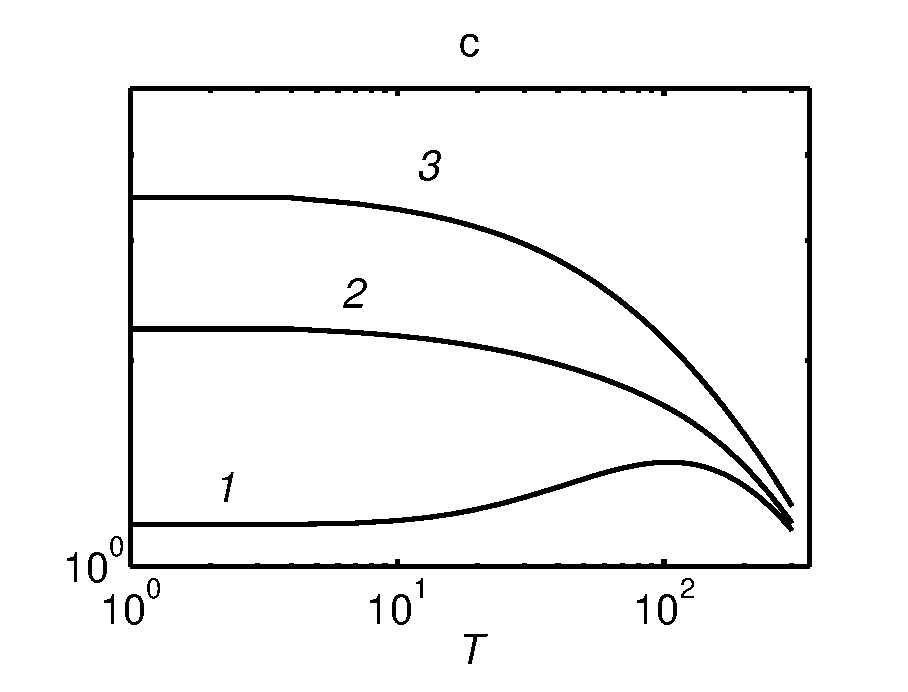
\includegraphics [scale=1] {fig_3_1_3}
\caption{Температурная зависимость подвижности (в относительных единицах) при учете рассеяния носителей на шероховатой поверхности и фононах в КЯ при $\Lambda =70 \AA$, $\Delta =3 \AA$, $L_{0}=100 \AA$, кривые 1, 2, 3 получены соответственно для $n_s = 10^{11} \text{cm}^{-2}$, $n_s = 7 \cdot 10^{11} \text{cm}^{-2}$, $n_s = 1.5 \cdot 10^{12} \text{cm}^{-2}$.} 
\label{img:syn_1}	
\end{figure}

На рисунке~\ref{img:syn_1} приведена температурная зависимость подвижности (в относительных единицах) для различных концентраций носителей в прямоугольной КЯ. Для невырожденного электронного газа (кривая 1) подвижность немонотонным образом зависит от $T$, что экспериментально наблюдалось в КЯ GaAs/AlAs \cite{Sakaki1987}, а также в КЯ Si/SiGe \cite{Yutani1996}. Заметим, что с ростом ширины КЯ уменьшается влияние рассеяния носителей на шероховатости поверхности, поэтому максимум подвижности смещается в область низких температур. Кривые 2, 3 описывают температурную зависимость подвижности для вырожденного электронного газа. При низких T подвижность практически не зависит от температуры и с ее ростом уменьшается. Именно такое поведение подвижности от температуры экспериментально наблюдалось в инверсионных слоях Si для вырожденного электронного газа \cite{Stern1980}.

Особый интерес представляет электропроводность в размерно-квантовых системах с учётом рассеяния носителей на шероховатой поверхности в магнитном поле. Направление и напряженность магнитного поля может существенным образом влиять на взаимодействие носителей с шероховатой поверхностью. 

Для случая $\vect{H} \parallel OX$, размерное квантование по $OZ$ получено выражение для электропроводнсти:
\begin{equation} \label{eq:syn_18}
\sigma_{xx} = \frac{e^2 k_0 T \hbar}{\pi \gamma_0 m_e L 4 V^2_0} \sum_n{\frac{\ln{\left\{\exp{\left[\beta \left(\widetilde{\xi}-\hbar \Omega n\right)\right]}+1\right\}}}{\left(n+\frac{1}{2}\right)}^2}. 
\end{equation}
Здесь
\[
\widetilde{\xi} = \xi -\frac{\hbar\Omega }{2}
\]
химический потенциал отсчитанный от дна нижайшей зоны проводимости, который находится из условия:
\begin{equation} \label{eq:syn_19}
N=\sum_{\alpha }{n_{\alpha}}.
\end{equation}
определяемый из уравнения:
\begin{equation} \label{eq:syn_20}
\sum_n{\ln{\left\{\exp{\left[\beta \left(\widetilde{\xi}-\hbar \Omega n\right)\right]}+1\right\}}}=\frac{\omega }{\Omega } \frac{\beta \hbar^2 \pi L n_e}{m_e}
\end{equation}
$n_e$~---~концентрация электронов.
Которое в квантовом пределе, когда все носители находятся на нижайшем уровне Ландау имеет вид:
\begin{equation} \label{eq:syn_21}
\mu _{xx} =\frac{4e\hbar }{m^2 \gamma } \left(\frac{\partial \omega }{\partial L} \right)^{-2} \left[1+\left(\frac{\omega_c}{\omega } \right)^2 \right]^{\frac{1}{2} }.
\end{equation}
Без учета рассеяния на шероховатой поверхности подвижность в размерно-ограниченных системах при учёте рассеяния носителей на длинноволновых колебаниях с ростом продольного магнитного поля уменьшается. Это связано с ростом локализации зонных электронов. В противоположность этому, как следует из \eqref{eq:syn_21} $\mu_{xx} $ в случае рассеяния на шероховатой поверхности с ростом магнитного поля увеличивается. Такое поведение зависимости подвижности от продольного магнитного поля может быть понято из следующих соображений. В параболической квантовой яме радиус локализации электрона $\lambda_0 =\sqrt{\hbar / (m\Omega) } $ с ростом напряженности магнитного поля уменьшается, число носителей тока, рассеивающихся на шероховатой поверхности размерно-ограниченной системы, становится меньше, что и приводит к росту подвижности.

Подвижность в поперечном магнитном поле при низких температурах для основного состояния, аналогично \eqref{eq:syn_21} имеет вид:
\begin{equation} \label{eq:syn_22}
\mu_{yy} =\frac{4e\hbar }{m^{2} \gamma } \left(\frac{\partial \omega }{\partial L} \right)^{-2} \left[1+\left(\frac{\omega _{c} }{\omega } \right)^{2} \right]^{-\frac{3}{2} }
\end{equation}
Следовательно, с ростом магнитного поля подвижность уменьшается и при
\[
\left(\frac{\omega_c}{\omega } \right)^2 \gg 1 \Rightarrow \mu_{xx} \sim \frac{1}{H} .
\]
Такое поведение подвижности от $H$ связано с тем, что в скрещенных магнитном и электрическом полях носители с дрейфовой скоростью перемещаются вдоль оси пространственного квантования по трохоиде, поэтому активно участвуют в процессах рассеяния на шероховатостях поверхности размерно-квантовой системы. 

Глава 4. Явления переноса в наноструктурах в поперечном электрическом поле с учетом рассеяния на шероховатой поверхности.

В 4.1 рассматривалось влияние постоянного поперечном электрического поля на рассеяние носителей на шеровховатой поверхности в параболической квантовой яме. В случае невырожденного электронного газа, при низких температурах, когда все носители находятся в нижайшей размерно-квантованной зоне проводимости $(n=0)$, подвижность определяется соотношением:
\begin{equation} \label{eq:syn_23}
\mu_{xx} =\mu_{xx}(0)\frac{1}{\left(1+2 N_c \right)^2 } ,
\end{equation}
где
\[
\mu_{xx}(0)=\frac{e}{m} \left(\frac{\hbar a^4 }{2\gamma_0 \Delta E_c } \right),
\]
подвижность в ПКЯ в отсутствии поперечного электрического поля.
Для параметров ПКЯ $(m_e = 0.06 m_0 )$ $\hbar \omega = 14.5/a_0 \text{ eV}$ ($a_0 $ --- ширина ПКЯ в ангстремах), $N_c =1.7\cdot 10^{-18} E_0^2 a_0^3 $ ($E_0 $ -- измеряется в V/cm). Таким образом, при $a_0 = 10^3 \AA$, $E_0 = 2.5\cdot 10^4 \text{ V/cm}$, $N_c =1$, подвижность уменьшается почти на порядок. С ростом $E$ носители тока «прижимаются» к одной из поверхностей квантовой ямы, поэтому их взаимодействие с шероховатой поверхностью увеличивается, что приводит к уменьшению времени релаксации, а следовательно и подвижности.

С ростом напряженности поперечного электрического поля минимум зоны проводимости смещается в запрещенную зону на $\Delta_c $, а экстремум валентной зоны поднимается на величину $\Delta_v =e^2 E^2  / (2m_v  \omega_v^2 )$ ($\hbar \omega_v $~---~шаг размерного квантования валентной зоны). Следовательно, ширина запрещенной зоны $E_g$ в рассматриваемой модели низкоразмерных систем уменьшается на $\Delta_c +\Delta_v $. Именно это обстоятельство приводит к тому, что с увеличением $E$ однозонное приближение при исследовании явлений переноса может оказаться не достаточным. В этом случае для расчета электропроводности необходимо учитывать нестандартность зоны проводимости \cite{Lax1960,Cohen1961}.

В 4.2 проводится расчеты подвижности для квантовой проволоки висмута в постоянно поперечном электрическом поле. Получено выражение для подвижности:
\begin{equation} \label{eq:syn_24}
\mu =\frac{\mu_0\sqrt{\pi } }{2\sum_{nm} F(\eta_{nm}^c )} \sum_{nm}\left\{\frac{\ln \left[\exp \left(\eta _{nm}^c \right)+1\right]}{\left(n+m+1+N_c \right)^2 } +\left(\frac{\Delta E_c }{\Delta E_v } \right)\frac{1}{p} \frac{\ln \left[\exp \left(\eta_{nm}^v \right)+1\right]}{\left(n+m+1+N_v \right)^2 } \right\} .
\end{equation}
Здесь введены обозначения:
\[
\mu_0 =\frac{4R^4 e}{\gamma \Delta E_c } \sqrt{\frac{k_0 T}{2\pi m_c } }, \;
R=\frac{a}{2}, \;
N_c =\frac{2\Delta_c }{\hbar \omega_c }, \;
N_v =\frac{2\Delta_v }{\hbar \omega_v },
\]
\[
\eta_{nm}^c =\frac{1}{k_0 T} \left[\xi -\hbar \omega_c \left(n+m+1\right)+\Delta_c \right],
\]
\[
\eta_{nm}^v =\frac{1}{k_0 T} \left[-\xi -\hbar \omega_v \left(n+m+1\right)+\Delta_0 +\Delta_v \right],
\]
\[
F(\eta_{nm}^c )=\int\limits_0^{\infty }{\frac{dx}{\exp \left(x^2 -\eta_{nm}^c \right)+1}}  ,
\]
$p$~---~число $c$ зон, участвующих в процессах электропроводности. Химический потенциал $\xi $ находится из условия электронейтральности исследуемой наноструктуры (число электронов в зонах проводимости равно числу дырок в валентной зоне)
\begin{equation} \label{eq:syn_25}
p\sqrt{\frac{m_c }{m_v } } \sum_{n,m}\int\limits_{0}^{\infty }{\frac{dx}{\exp \left(x^2 -\eta_{nm}^c \right)+1}}  =
\sum_{n,m}\int\limits_0^{\infty}{\frac{dx}{\exp \left(x^2 -\eta_{nm}^v \right)+1}}.
\end{equation}
Положение химического потенциала при заданных параметрах наносистемы определяется величиной радиуса $R$ квантовой проволоки и величиной напряженности поперечного электрического поля.

\begin{figure}[!h]
\center
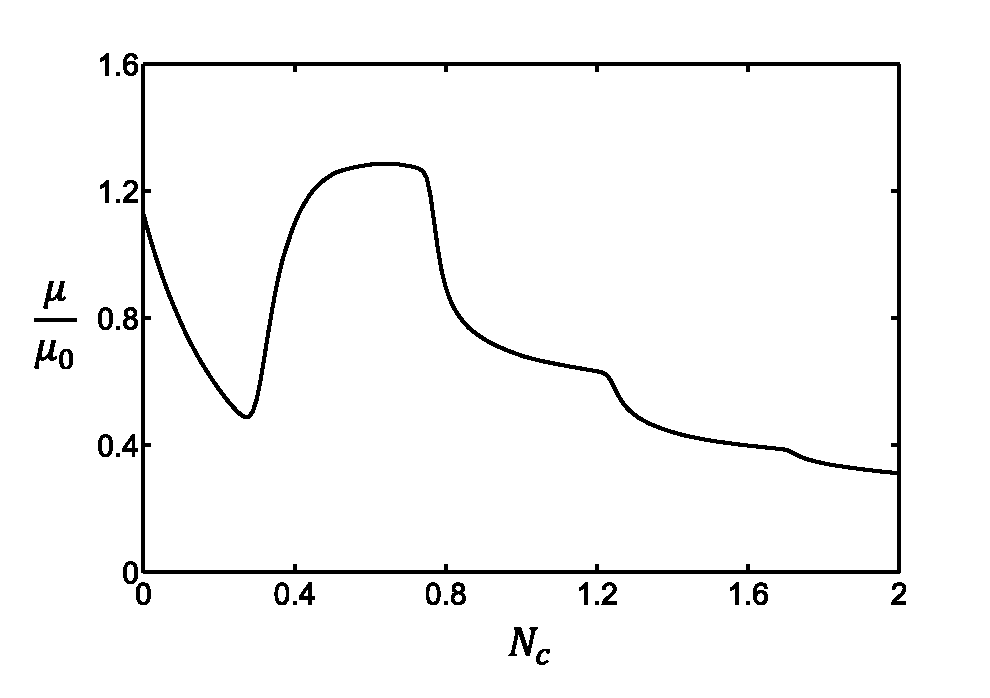
\includegraphics [scale=0.8] {fig_4_2_2}
\caption{Зависимость подвижности (в относительных единицах) от напряженности поперечного электрического поля. $R=330 \AA$.}
\label{img:syn_2}
\end{figure}

Влияние поперечного электрического поля на подвижность принципиальным образом зависит от радиуса нанопроволоки. При небольших значениях $R$, когда квантовая проволока представляет почти безщелевой полупроводник, с ростом $E$ (при $E=0$ электронный (дырочный) газ невырожден) подвижность сначала уменьшается, затем увеличивается, и в дальнейшем описывается осцилляционной кривой (рисунок~\ref{img:syn_2}). Такое поведение подвижности в присуствии поперечного электрического поля связано с тем, что с ростом напряженности поперечного электрического поля, дно размерно-квантованных $c$ зоны, опускаясь в область запрещенных значений энергии, пересекает химический потенциал, что приводит к увеличению подвижности. Заметим, что для типичных значений параметров нанопроволок Bi ($m_c = 0.01m_0 $, $m_v = 0.1m_0$, $\Delta E_c  / \Delta E_v  = 1.5$) $N_v =5.8 N_c $, поэтому с ростом $E$ влияние дырок на поведение $\mu$ от $E$ слабее, чем для электронов. Следовательно, осцилляционная зависимость подвижности от $E$ должна наблюдаться и для полупроводниковых квантовых проволок с вырожденным электронным газом.

\begin{figure}[!h]
	\center
	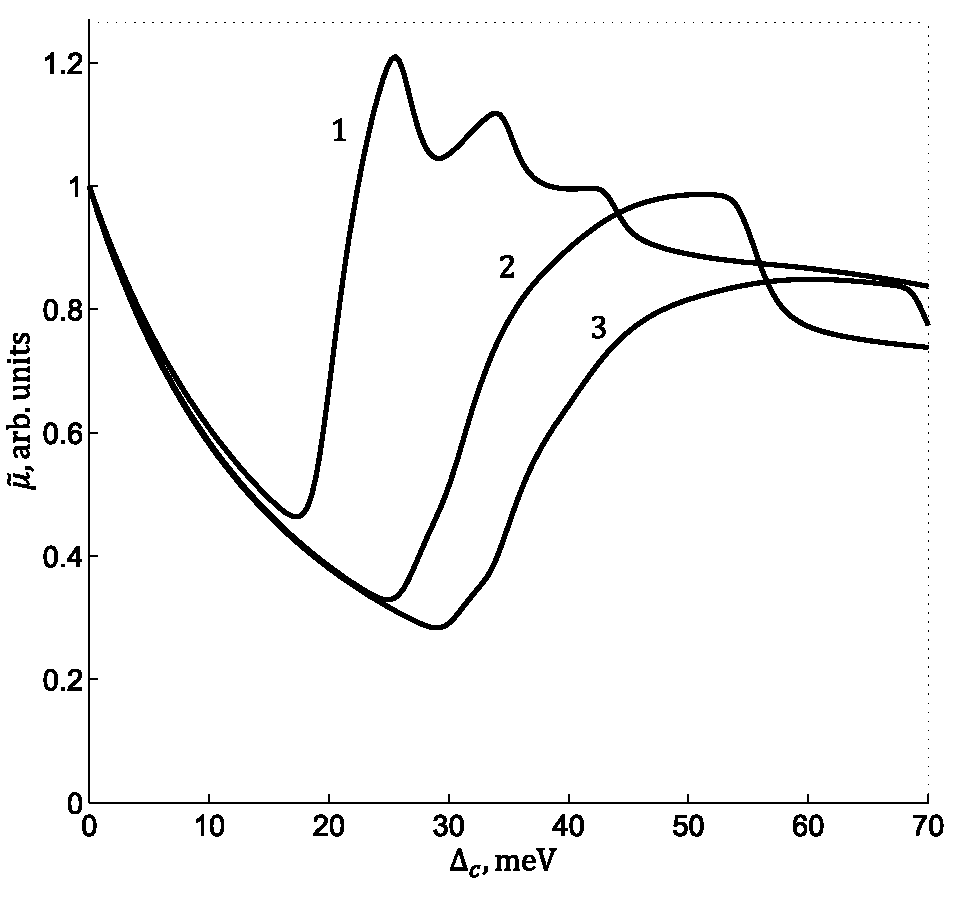
\includegraphics [scale=0.8] {fig_4_3_1}
	\caption{Зависимость подвижности в относительных единицах $\widetilde{\mu}=\mu(E)/\mu(0)$ от электрического поля.}
	\label{img:syn_3}
\end{figure}

В 4.3 рассмотренно влияние рассеяния носителей тока на шероховатой поверхности в нанопроволоках в поперечных электрическом и магнитном полях
Для этого случая получено соотношение для электропроводности :
\begin{equation} \label{eq:syn_26}
\sigma_{xx}=\frac{2 e^2\hbar}{\beta_0 \pi^2 m^*_x \gamma_0} \sum_{nm}{\frac{\ln \left[1+\exp\left(\beta_0 \xi_{nm}\right)\right]}{\left[\hbar \omega_y \frac{\omega_y}{\Omega_y}\left(n+\frac{1}{2}\right)+\hbar \omega_z\left(m+\frac{1}{2}\right)+2\Delta_c\right]^2}}
\end{equation}
\[
\xi_{nm}=\xi -\hbar \Omega_y \left(n+\frac{1}{2}\right)-\hbar \omega_z\left(m+\frac{1}{2}\right)+\Delta_c,\;
\beta =\frac{1}{k_0 T}
\]
$\xi $~---~химический потенциал исследуемой наносистемы. Аналогично можно записать $\sigma_{xx}$ для дырок в валентной зоне полуметалла Bi. В этом случае в эффективные массы электронов нужно заменить на соответствующие массы дырок $\mu_x,\; \mu_y,\; \mu_z$, а $\xi$  на $-\xi +\Delta_0$ ($\Delta_0$ определяется перекрыванием валентной зоны и зоны проводимости, $\Delta_0\cong 39\text{ meV}$ \cite{Levin2009a}).

На рисунке~\ref{img:syn_3} приведены численные расчеты зависимости подвижности (в относительных единицах) от напряженности поперечного электрического поля. Кривые 1, 2, 3 получены при $\delta = 0$, $\delta = 0.05$, $\delta = 0.1$ соотвественно $\left(\delta = {\left(\omega^c_x/\omega_y\right)}^2\right)$. При малых значениях $\Delta_c$ электронный газ (при рассмотренных параметрах квантовой проволоки) является невырожденным, поэтому с ростом напряженности поперечного электрического поля подвижность уменьшается. Кривая 1 (подвижность в отсутствии  магнитного поля $\delta = 0$) описывается тремя максимумами. Такая осцилляционная зависимость подвижности связана с тем, что с ростом $E$ химический потенциал, отсчитанный от дна размерно-квантованной зоны проводимости, поднимается в область больших значений энергии и может пересечь дно размерно-квантованной $c$ зоны, в которой существуют особенности в плотности энергетических состояний. Первый пик связан с пересечением химического потенциала нижайшего состояния размерно-квантованной $c$ зоны $(n=0,\; m=0)$, второй пик возникает из-за пересечения химического потенциала дна первой размерно-квантованной зоны $(m=0,\; n=1)$, третий пик -- из-за пересечения химического потенциала второй размерно-квантованной зоной $(m=1,\; n=0)$. С ростом напряженности магнитного поля дно размерно-квантованной зоны проводимости поднимается в область больших значений энергии, поэтому пересечение химического потенциала наступает при больших значениях $\Delta_c$. Именно по этой причине первый пик кривой 2 сдвинут по отношению первого пика кривой 1 в область больших значений напряженности поперечного электрического поля.


\ifdefmacro{\microtypesetup}{\microtypesetup{protrusion=false}}{} % не рекомендуется применять пакет микротипографики к автоматически генерируемому списку литературы
\ifnumequal{\value{bibliosel}}{0}{% Встроенная реализация с загрузкой файла через движок bibtex8
  \renewcommand{\bibname}{\large \authorbibtitle}
  \nocite{*}
  \insertbiblioauthor           % Подключаем Bib-базы
  %\insertbiblioother   % !!! bibtex не умеет работать с несколькими библиографиями !!!
}{% Реализация пакетом biblatex через движок biber
  \ifnumgreater{\value{usefootcite}}{0}{
%  \nocite{*} % Невидимая цитата всех работ, позволит вывести все работы автора
  \insertbiblioauthorcited      % Вывод процитированных в автореферате работ автора
  }{
  \insertbiblioauthor           % Вывод всех работ автора
%  \insertbiblioauthorgrouped    % Вывод всех работ автора, сгруппированных по источникам
%  \insertbiblioauthorimportant  % Вывод наиболее значимых работ автора (определяется в файле characteristic во второй section)
  \insertbiblioother            % Вывод списка литературы, на которую ссылались в тексте автореферата
  }
}
\ifdefmacro{\microtypesetup}{\microtypesetup{protrusion=true}}{}

